%! Author = joaopintosp
%! Date = 8/25/24

\section{Resultados}\label{sec:resultados}

\subsection{Discussão de Resultados}\label{subsec:discussao}

Ou seja, quando for possível acabar com isto.
Espero que seja possível alterar isto de forma a que isto seja viável.
Com o Vim seria capaz de aumentar o meu ritmo de escrita considerávelmente.
Nesta secção iremos apresentar os resultados da nossa pesquisa e analisar os dados obtidos.
Normalmente, num trabalho de investigação, isto tem de ser feito de forma a corroborar as conclusões que irão ser tomadas nas secções finais do presente documento.

Nesse sentido, apresenta-se os seguintes resultados:

\begin{table}[htb!]
    \centering
    \caption{Resultados obtidos.}
    \label{tab:tabela1}
    \begin{tabular}{|c|c|c|}
        \hline
        1 & 2 & 6 \\ \hline
        3 & 4 & 7 \\ \hline
    \end{tabular}
\end{table}

\subsection{Cálculos efetuados}\label{subsec:calculos}

Nesta secção iremos falar sobre os resultados obtidos e apresentados na secção anterior e iremos apresentar os cálculos que nos permitiram chegar a tais resultados.

Começa-se por uma descrição dos trabalhos realizados:
\begin{enumerate}
    \item Perceber o teatro;
    \item Tentar resolver o teatro;
    \item Aperceber-se que não se sabe resolver o teatro;
    \item Desistir de resolver o teatro;
    \item Perguntar ao ChatGPT a resposta;
    \item Discutir os resultados como se fosse eu que os tivesse feito.
\end{enumerate}

\paragraph{Um Diagrama:} Vamos agora observar um diagrama que representa o problema:

\begin{figure}[htb!]
    \centering
    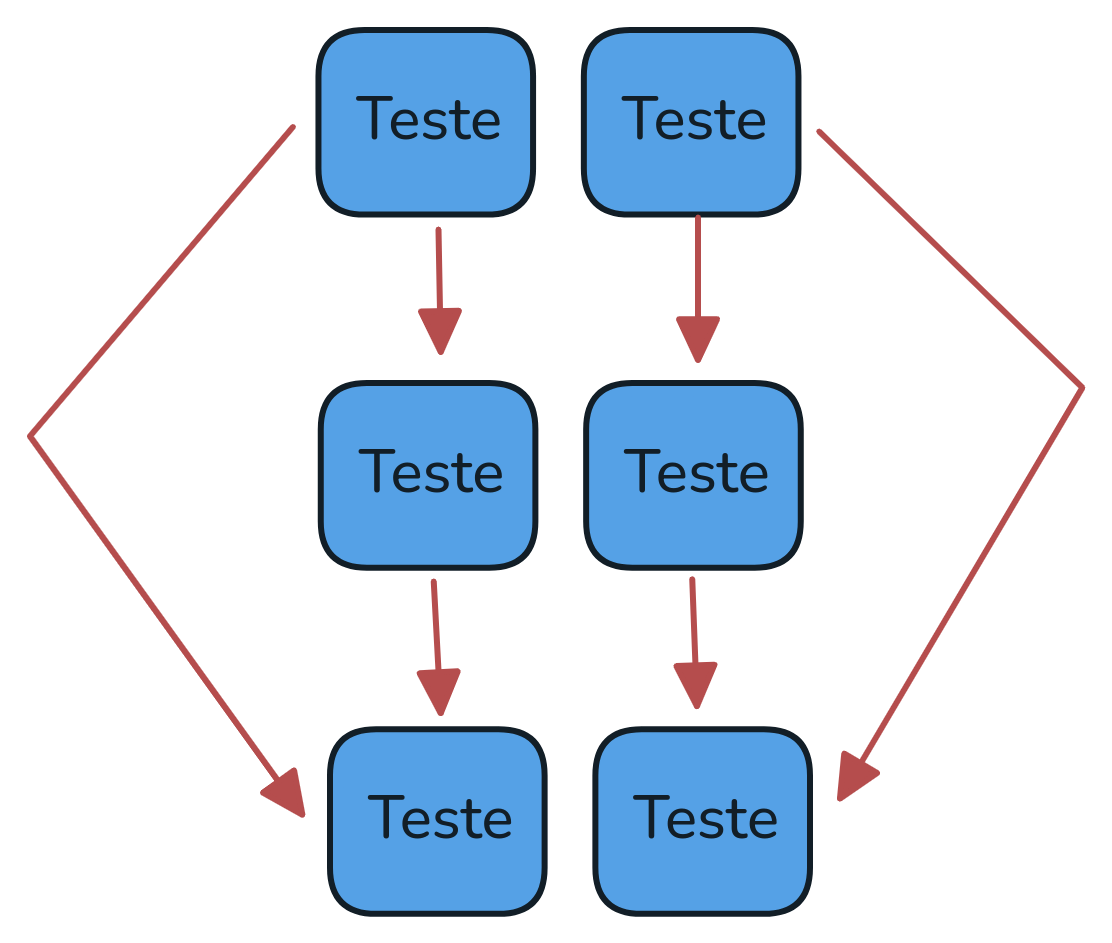
\includegraphics[width=0.5\textwidth]{figures/teste}
    \caption{Isto é apenas um teste.}
    \label{fig:teste}
\end{figure}

\begin{figure}[htb!]
    \centering
    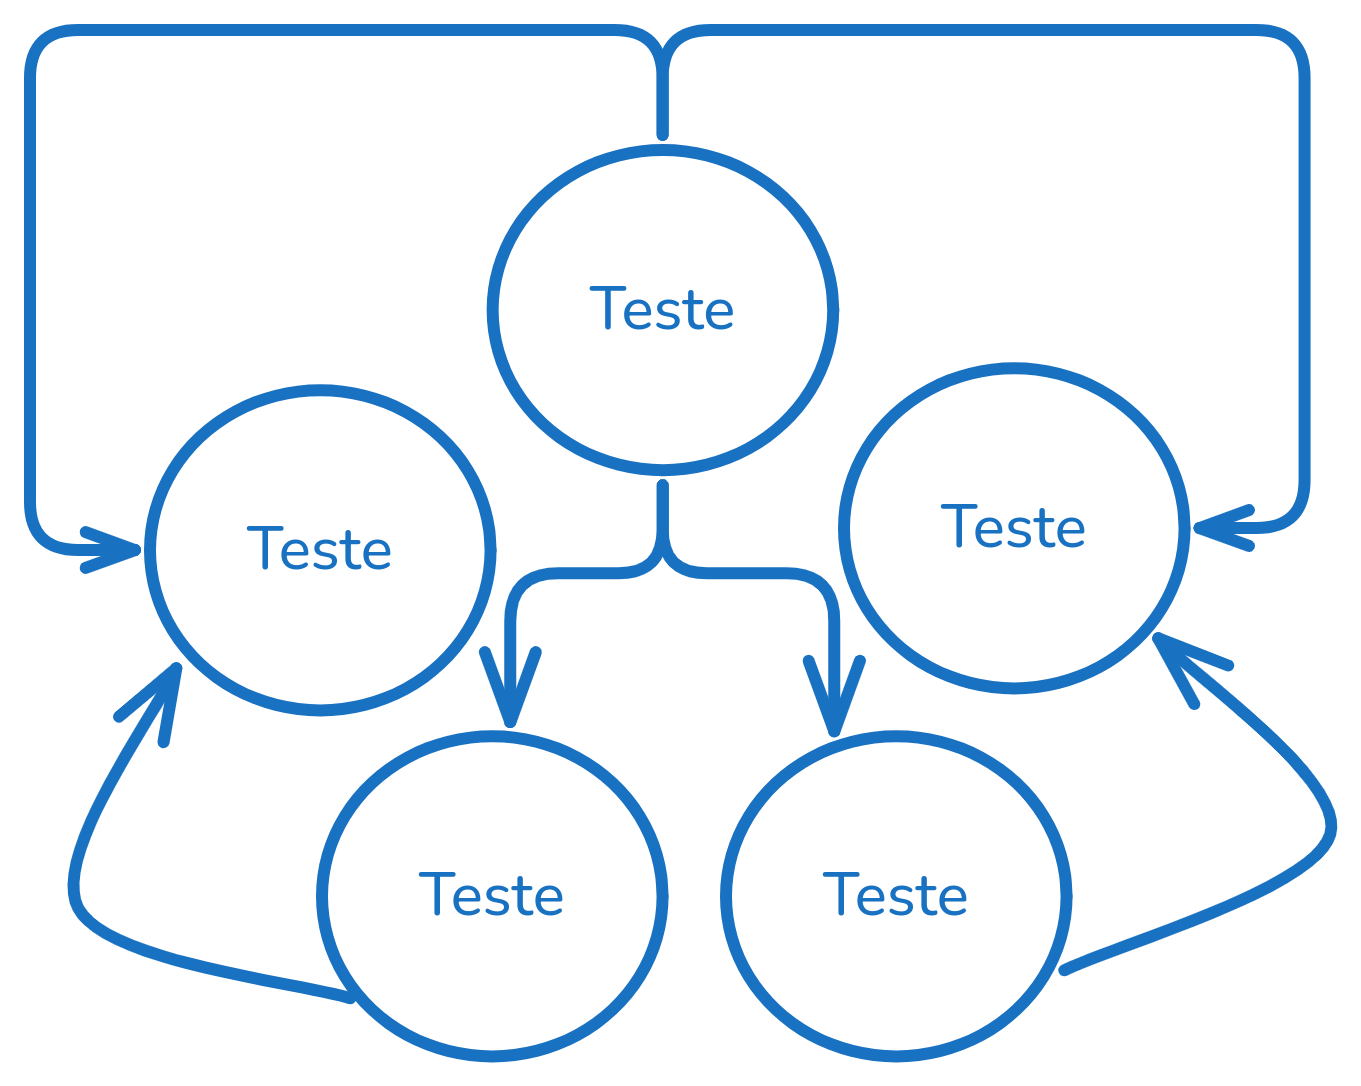
\includegraphics[width=0.5\textwidth]{figures/diagrama}
    \caption{Isto é apenas um teste.}
    \label{fig:diagrama}
\end{figure}

Como podemos ver pelas figuras anteriormente apresentadas, a Figura~\ref{fig:teste} é azul e a Figura~\ref{fig:diagrama} é azul com obrigado.
